\section{Results}
\label{sec:results}

\subsection{Comparison with a supervised baseline}
\label{sec:comparison}

\begin{table}[t]
\centering
\small
\caption{Shared test set, same pixels and targets for both models. Bold marks the better of a pair when the two differ by 3\% or more; we have no seed spread, so smaller differences count as ties, as do pairs of percentiles one histogram bin (0.02\,dex) apart. Lower is better except in the last two rows, where the target is the solver's own value: 100\% for emission and, for 94\Ang, 92\% on BP and 55\% on Elastic Net.}
\label{tab:headline}
\begin{tabular}{@{}lcccc@{}}
\toprule
 & \multicolumn{2}{c}{Basis Pursuit} & \multicolumn{2}{c}{Elastic Net}\\
\cmidrule(lr){2-3}\cmidrule(l){4-5}
Measure & Ours & Sup. & Ours & Sup.\\
\midrule
DEM MAE & \textbf{0.072} & 0.100 & \textbf{0.151} & 0.188\\
DEM MSE & 1.08 & \textbf{0.91} & 0.310 & 0.318\\
EM error (\%) & \textbf{11.0} & 14.3 & \textbf{12.2} & 18.0\\
W1 (dex) & \textbf{0.070} & 0.133 & \textbf{0.103} & 0.121\\
AIA MAE (DN/s) & 3.54 & \textbf{2.95} & \textbf{0.56} & 6.32\\
AIA MSE & \textbf{148} & 157 & \textbf{161} & 598\\
\midrule
Median pixel error & \textbf{0.031} & 0.112 & \textbf{0.85} & 1.12\\
p90 & 1.86 & 1.95 & \textbf{7.76} & 8.51\\
p99 & 25.7 & 26.9 & \textbf{29.5} & 35.5\\
p99.9 & 170 & 162 & \textbf{102} & 178\\
\midrule
Quiet MSE & 0.0331 & 0.0335 & \textbf{0.122} & 0.130\\
MSE without flare cores & \textbf{0.087} & 0.091 & \textbf{0.172} & 0.210\\
Flare-core emission (\%) & \textbf{96.7} & 92 & \textbf{99} & 87\\
Flare-core 94\Ang{} (\%) & 88 & 85 & \textbf{53} & 48\\
\bottomrule
\end{tabular}
\end{table}

\Cref{tab:headline} compares our final models with the supervised baseline. On Elastic Net our model leads on five of the six headline measures and ties on DEM MSE (0.310 against 0.318). Its AIA MAE is eleven times lower than the baseline's and also lower than the solver's own 1.41\,DN/s, though the solver's AIA MSE (134) is lower than ours. That tie depends on a test-informed choice: at 120 epochs, which the validation loss preferred, our DEM MSE is 0.362 and the baseline would lead.

On BP our model leads on four of the six, and the baseline keeps DEM MSE (0.91 against 1.08) and AIA MAE (2.95 against 3.54). BP's own AIA MAE on these pixels is 4.26\,DN/s, worse than either network, because the solver only has to land inside the band, while its AIA MSE (61.9) beats both. The BP mean and median disagree because the error is heavy-tailed. On the typical pixel our model is 3.6 times closer to the solver (0.031 against 0.112), and from the 90th percentile upward the two are level within the resolution of our histograms. Flare cores, one pixel in 10,000, hold 92.0\% of our squared error and 90.0\% of the baseline's. Without them our DEM MSE is slightly lower (0.087 against 0.091), so the BP DEM MSE gap comes from flare cores, where our error is 1.22 times the baseline's.

The clearest differences between the two models are in shape, which the means hide. At BP flare cores the baseline falls 10\% to 22\% short of the observed 131 to 211\Ang, while ours stays within 1\% (\cref{tab:channels}). The baseline flags 41.1\% of pixels as multi-peaked at 24\% precision against the solver, and ours flags 12.8\% at about 63\%, with the solver itself at 13.5\%. W1, which measures where emission sits in temperature, is about half the baseline's.

The five targets also bound what any deterministic model can do. Where several targets cover a block, the MSE splits into the distance to the mean solver DEM and the solver's own scatter across re-solves. For our BP model that scatter is 43.9\% of the Quiet error and 0.3\% of the flare-core error. Nearly half of the remaining Quiet error is the solver disagreeing with itself under half-$\sigma$ noise, while the flare-core error belongs to the model.

\subsection{The flare-core failure was in the loss}
\label{sec:flare}

\begin{figure}[t]
  \centering
  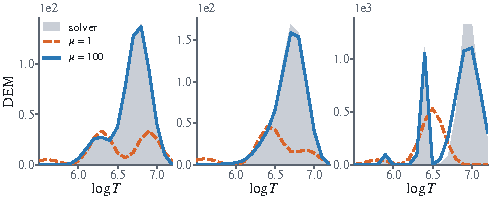
\includegraphics[width=\linewidth]{fig_curves.pdf}
  \caption{Three random flare cores from validation, among those with a solved LP and a binding 94\Ang{} lower edge: the solver's DEM against the numerical minimizer of the loss. At $\mu=1$ the hot peak disappears. No network is involved.}
  \label{fig:curves}
\end{figure}

\begin{table*}[t]
\centering
\small
\caption{BP runs on the shared test set. Flare-core columns are percentages (solver: 100 and 92). The bold row is the final model, the only one with channel masking; every other label-free row drops clamped pixels. The 360k model uses a logarithmic input and all others the square-root Fourier input.}
\label{tab:runs}
\setlength{\tabcolsep}{4.5pt}
\begin{tabular}{@{}llccccccc@{}}
\toprule
Loss & Model & Epochs & DEM MSE & Median & AIA MSE & Quiet MSE & Emission & 94\Ang\\
\midrule
$\mu=1$ & 360k & 40 & 4.28 & 0.026 & 83 & 0.058 & 40 & 23\\
 & 409k & 40 & 4.56 & 0.023 & 83 & 0.057 & 35 & 15\\
 & 409k, flare cores oversampled & 40 & 5.05 & 0.025 & 87 & 0.058 & 24 & 9\\
 & 409k & 120 & 4.21 & 0.022 & 108 & 0.057 & 37 & 16\\
 & 10M & 40 & 5.10 & 0.022 & 125 & 0.058 & 20 & 8\\
\midrule
$\mu=100$ & 409k & 40 & 2.37 & 0.062 & 44 & 0.035 & 89 & 68\\
 & 409k & 120 & 2.00 & 0.041 & 44 & 0.032 & 92 & 75\\
 & 409k & 120+120 & 1.75 & 0.036 & 103 & 0.032 & 93 & 77\\
 & 1.5M & 120 & 897 & 0.034 & 21.7M & 12.5 & 115 & 78\\
 & \textbf{1.5M, channels masked} & \textbf{120} & \textbf{1.08} & \textbf{0.031} & \textbf{148} & \textbf{0.033} & \textbf{97} & \textbf{88}\\
\midrule
$\mu=300$, solver's band & 409k & 120 & 1.54 & 0.045 & 116 & 0.050 & 97 & 87\\
\midrule
\multicolumn{2}{@{}l}{Supervised baseline} & & 0.91 & 0.112 & 157 & 0.033 & 92 & 85\\
\bottomrule
\end{tabular}
\end{table*}

At $\mu=1$ our first production model reproduced 171, 193 and 211\Ang{} at flare cores to within 2\%, but only 23\% of 94\Ang, 76\% of 131\Ang{} and 67\% of 335\Ang, the channels that see hot plasma, and it held 40\% of the solver's emission. The natural reading is underfitting. \Cref{tab:runs} shows the three obvious remedies on the original loss. Oversampling raised flare cores 8.4-fold in training and made them worse, tripling the epochs moved flare-core emission from 35\% to 37\%, and a 10M-parameter model reached 20\%.

\begin{table}[t]
\centering
\small
\caption{Four answers scored under the original loss ($\mu=1$) at validation flare cores: total loss, its sparsity and penalty terms, the share of observed 94\Ang{} reproduced, and emission relative to the solver.}
\label{tab:gap}
\begin{tabular}{@{}lcccc@{}}
\toprule
Answer & Loss & Sparsity + penalty & 94\Ang & EM\\
\midrule
Network, $\mu=1$ & 565 & 294 + 270 & 28\% & 38\%\\
Minimizer $w^\circ$ & 463 & 220 + 243 & 26\% & 30\%\\
Solver's DEM & 1,125 & 1,119 + 6 & 94\% & 100\%\\
Supervised DEM & 1,878 & 1,107 + 771 & 91\% & 95\%\\
\bottomrule
\end{tabular}
\end{table}

\Cref{tab:gap} gives the diagnosis. The amortization gap was small: the network's median loss sits 8.0\% above the per-pixel minimum at flare cores and 0.8\% to 3.6\% above it from 0.03 to 32 times the Bright cutoff, so training had converged. The minimizer itself reproduces only 26\% of 94\Ang. The loss rates the solver's DEM 2.4 times worse than an answer without the hot plasma, so better training on this loss cannot recover it. \Cref{fig:curves} shows the effect at three random flare cores. The original weight was outside the law's range: $\mu_0$ exceeds 1 at 99.9\% of solved flare cores. Extrapolating the first linear piece of \cref{eq:path}, a hot element ($\logT\ge6.6$) reaches zero above $\mu=1$ at 96\% of them, with a median of 10.6.

Raising $\mu$ to 100 restores the hot plasma at feasible pixels. With only that change, DEM MSE halves and flare-core emission rises from 35\% to 89\%. Training then becomes the limit: at flare cores the amortization gap is 118\% after 40 epochs and 47\% after 120. Longer training and greater capacity close most of the rest (\cref{tab:runs}). The final model holds 96.7\% of the solver's emission at flare cores and reproduces 88\% of 94\Ang, against 92\% for the solver and 85\% for the baseline.

The same mechanism explains a milder effect at ordinary pixels. Nothing pulls a channel toward its observation inside the band, so the sparsity term drags emission to the band's lower edge, and a finite $\mu$ lets it slip past. At 0.3 to 1 times the Bright cutoff the minimizer emits 0.861 of the solver's emission at $\mu=1$ and 1.009 at $\mu=100$. Over the test set, emission relative to the solver rose from 0.848 for our first model to 0.988 for the final one.

\subsection{Testing the penalty law}
\label{sec:verify}

\begin{figure*}[t]
  \centering
  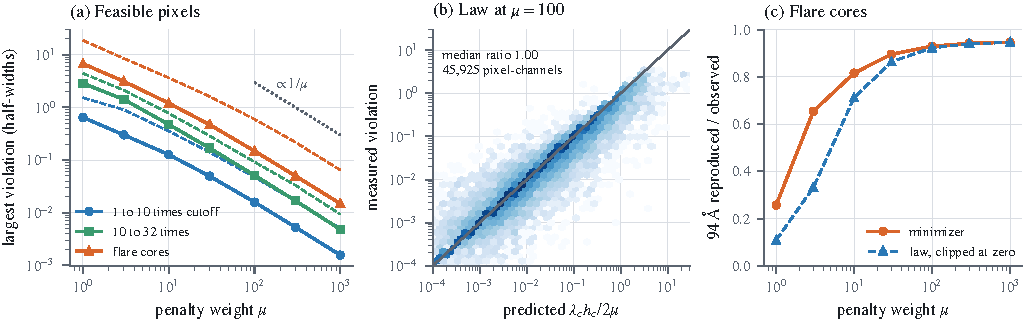
\includegraphics[width=\linewidth]{fig_law.pdf}
  \caption{The penalty law on validation pixels. (a) Largest violation per pixel against $\mu$ at pixels with a solved LP: median (solid) and 90th percentile (dashed), by brightness relative to the Bright cutoff. (b) Measured against predicted violation at $\mu=100$ for every pixel-channel above $10^{-4}$ half-widths. (c) 94\Ang{} reproduced at 4,863 solved flare cores where the 94\Ang{} lower edge binds: the loss's numerical minimizer against \cref{eq:law} using each pixel's LP price, clipped as in \cref{eq:clip}.}
  \label{fig:law}
\end{figure*}

\begin{table}[t]
\centering
\small
\caption{The law by brightness band (multiples of the Bright cutoff) on validation pixels: pixels sampled, share with a solved LP, the median threshold $\mu_0$ of \cref{prop:law}, the share with $\mu_0\le100$, and the $\mu$ that holds the median and the 90th-percentile pixel within 0.1 half-widths.}
\label{tab:law}
\begin{tabular}{@{}lrcccrr@{}}
\toprule
Band & Pixels & Solved & $\mu_0$ & $\le100$ & \multicolumn{2}{c}{$\mu$ for 0.1}\\
\midrule
$<0.03$ & 50 & 100\% & 0.06 & 100\% & 0.2 & 0.4\\
0.03--0.1 & 296 & 99\% & 0.11 & 100\% & 0.3 & 1.4\\
0.1--0.3 & 608 & 99\% & 0.20 & 99\% & 0.6 & 2.5\\
0.3--1 & 1,000 & 94\% & 1.5 & 92\% & 2.3 & 21\\
1--1.8 & 1,000 & 88\% & 8.1 & 87\% & 11 & 44\\
1.8--3.2 & 1,000 & 90\% & 7.6 & 87\% & 13 & 48\\
3.2--10 & 1,000 & 96\% & 10 & 84\% & 25 & 68\\
10--32 & 1,000 & 100\% & 15 & 87\% & 53 & 102\\
$\ge 32$ & 6,000 & 88\% & 37 & 72\% & 168 & 763\\
\midrule
All & 11,954 & 91\% & 18 & 81\% & 64 & 367\\
\bottomrule
\end{tabular}
\end{table}

We solved the LP and the loss at seven values of $\mu$ from 1 to 1,000 on 11,954 validation pixels, 6,000 of them flare cores. The LP has a solution at 10,899 of them, and all but 29 of those are nondegenerate (\cref{tab:law}).

\Cref{prop:law} makes a sharp prediction, because $\mu_0$ can be computed for each pixel from the LP before any penalized solve. Above $1.05\,\mu_0$ the law should hold, and well below it should not. That is what we find. At $\mu=1$, 99.4\% of pixel-channels above their threshold are within 5\% of the prediction, against 3.7\% of those below $0.5\,\mu_0$. The median ratio above the threshold is 1.00 at every $\mu$, and below it 0.49 to 0.70. The share within 5\% falls to 85\% at $\mu=100$ and 68\% at $\mu=1{,}000$, but these misses are optimizer error: at all of the 1,299 and 3,036 pixels involved, \cref{eq:path} has a loss no higher than the L-BFGS-B answer. Over the 45,925 pixel-channels violated at $\mu=100$ the median ratio is 1.00 (\cref{fig:law}b).

\Cref{tab:law} shows that the threshold is low enough to matter in practice. The median $\mu_0$ is below 2 up to the Bright cutoff and 37 at flare cores, and 72\% of solved flare cores have $\mu_0\le100$. Median violations at flare cores fall with a slope of $-0.7$ at small $\mu$ and reach $-1$ from about $\mu=30$ (\cref{fig:law}a). Using LP prices alone, the law reproduces the 94\Ang{} column of the screen from $\mu=30$ upward (0.923 predicted, 0.930 measured at $\mu=100$). At small $\mu$ it underestimates that column (0.11 against 0.26 at $\mu=1$), as expected once the solution has changed support (\cref{fig:law}c). The one-element threshold \eqref{eq:drop} is therefore a guide to scaling rather than a pixel-level predictor. Its median at flare cores is 1.32, against 37 for the exact $\mu_0$.

The prices match \cref{sec:law}. At flare cores the median 94\Ang{} price is 1.46, close to the single-edge value of 1.48, although every solved flare core binds three to six edges. It exceeds that value at 49\% of them (99th percentile 8.8). 94\Ang{} has the largest predicted violation at 70\% of flare cores, 335\Ang{} at 15\% and 131\Ang{} at 13\%. With measured prices $\mudrop$ exceeds 1 for 131\Ang{} at 17\% of solved flare cores, and for 193 and 335\Ang{} at 3\%. The noise ratio behaves as \cref{eq:drop-shot} assumes: in 94\Ang{} at flare cores $g$ runs from 0.806 to 0.817 between the 10th and 90th percentiles.

The screen in \cref{tab:screen} kept $\mu=100$ before we had the law, and the law says what that choice means. At $\mu=100$ the median solved flare core sits 0.15 half-widths outside its band and the 90th percentile 0.60 (predicted 0.17 and 0.76). The value of 120 that \cref{sec:law} obtains from $R$ and the noise alone is close to where the screen's 94\Ang{} column levels off. A single $\mu$ cannot hold every pixel to one tolerance: the hardest solved pixel in the sample, a flare core priced on 335\Ang, would need 63,801 for 0.1 half-widths.

The law describes the minimizer rather than the network, and a network adds its amortization gap on top. At validation flare cores the 409k model at $\mu=100$ (120+120 epochs) has a median worst-channel violation of 0.79 half-widths against the minimizer's 0.18, with a maximum of 1,695. We have not made this measurement on the final model.

\subsection{Pixels where no DEM fits the band}
\label{sec:infeasible}

\begin{table}[t]
\centering
\small
\caption{The screen on validation: the loss's minimizer, with no network, scored against the solver. DEM error is the DEM MSE with brightness bands weighted by population. ``Fixed'' keeps the $1.4\sigma$ band everywhere and ``Solver'' widens it where the solver did. Supervised reference: DEM error 6.10, Quiet MSE 0.054.}
\label{tab:screen}
\setlength{\tabcolsep}{4.5pt}
\begin{tabular}{@{}rcccccc@{}}
\toprule
 & \multicolumn{2}{c}{DEM error} & \multicolumn{2}{c}{Quiet MSE} & \multicolumn{2}{c}{Flare core, fixed}\\
\cmidrule(lr){2-3}\cmidrule(lr){4-5}\cmidrule(l){6-7}
$\mu$ & Fixed & Solver & Fixed & Solver & 94\Ang & EM\\
\midrule
1 & 36.9 & 37.8 & 0.076 & 0.074 & 26\% & 30\%\\
10 & 10.9 & 12.1 & 0.037 & 0.027 & 81\% & 90\%\\
30 & 4.94 & 5.47 & 0.034 & 0.015 & 89\% & 97\%\\
100 & 2.30 & 2.79 & 0.046 & 0.0079 & 93\% & 100\%\\
300 & 1.78 & 1.11 & 0.053 & 0.0036 & 94\% & 101\%\\
1000 & 2.17 & 0.63 & 0.055 & 0.0018 & 95\% & 101\%\\
\bottomrule
\end{tabular}
\end{table}

The fixed-band columns of \cref{tab:screen} show a trade-off. Raising $\mu$ first helps and then hurts, and faint-pixel error climbs from $\mu=30$ upward. The cause is one group of pixels. At 8.8\% of the sample, and 12\% of flare cores, the LP has no solution at the $1.4\sigma$ band: 7.8\% are provably infeasible and the rest are numerical failures of the LP solver. These are the pixels the reference solver relaxes. There the violation has a floor set by the observation, and raising $\mu$ pushes the minimizer away from the solver. At 0.3 to 1 times the Bright cutoff its DEM error at those pixels grows from 0.055 at $\mu=1$ to 0.92 at $\mu=100$ and 1.29 at $\mu=1{,}000$. At $\mu=100$ they hold 70\% to 90\% of the minimizer's error between 0.3 and 10 times the cutoff.

Widening the band where the solver widened it, while still measuring the excess in units of the original half-width, removes the trade-off. Every column in \cref{tab:screen} then improves monotonically with $\mu$, and a perfect network would simply want the largest $\mu$.

A real network does not get there. We trained the 409k model for 120 epochs at $\mu=300$ on the solver's band (\cref{tab:runs}). At the targeted pixels it did what the screen predicts, with validation DEM MAE of 0.15 against 0.45 for the same recipe at $\mu=100$, and it improved test DEM MSE and flare-core 94\Ang{} (1.54 and 87\%, against 2.00 and 75\%). But test Quiet MSE rose to 0.050, far above the 0.0036 the minimizer reaches on validation, and one validation pass spiked to $4\times10^{16}$. The loss had improved and the optimization had become harder, a pattern familiar from stiff penalties in physics-informed networks~\cite{wang2021pathologies,krishnapriyan2021failure}. Widening also needs the solver's per-pixel flag, or an LP feasibility check per pixel, which gives back part of what label-free training saves. We therefore keep the fixed band at $\mu=100$, and the final model reaches the same flare-core quality that way. A 1.5M model on the widened band remains untested. Because the BP test targets are missing at these pixels, the headline scores can show neither the gain from widening nor the cost of not widening.

\subsection{Capacity and out-of-distribution inputs}
\label{sec:capacity}

With clamped pixels dropped from training, wider models improved the typical pixel and failed by orders of magnitude on a few others. On Elastic Net with a logarithmic input, models of 722k and 1.43M parameters reached DEM MSE 3.24 and 36.2 against 0.48 at 360k, and with our final input a 10M model reached 2,062 against 0.310 at 409k. The validation loss preferred or tied each of them. On BP at $\mu=100$ a 1.5M model has a median pixel error of 0.034 and a DEM MSE of 897, with 99.7\% of its squared error in its worst 100 of 705M pixels.

Most of these failures share a cause. In those Elastic Net models and the 10M BP model, 93\% to 99\% of the squared error sits in pixels with a clamped channel. The failing inputs are strange. In the 1.5M model's worst 100 distinct inputs a median of five of six channels read at most $10^{-3}$\,DN/s, and in 56\% a single channel has signal, always 94\Ang, at a median 3.0\,DN/s and 28 times the median of its eight neighbors. Such a lone reading looks like a residual cosmic-ray hit or a hot pixel. Our training mask had removed every pixel with a clamped channel, 40\% of pixels rather than the 5\% we first estimated from two channels, and the validation loss used the same mask, so neither had ever contained such an input. In standardized log intensity these inputs sit about 4.9 from the nearest of 2M training pixels, while test pixels above 0.3 times the cutoff sit 0.08 to 0.21 away. Near the data the loss pins the output, and far from it nothing does~\cite{hein2019relu,xu2021extrapolate}. A larger network has more room to bend there: over the 10M Elastic Net model's worst 1,000 inputs the median emission is $1.6\times10^5$ times the solver's. Distance alone does not mark failure, though, since faint pixels can sit as far out without any error.

Channel masking (\cref{sec:clamp}) tests this account. It takes the 10M Elastic Net model from DEM MSE 2,062 to 1.82, though that model keeps an AIA MSE of 148,403, and it brings the 1.5M BP model's Quiet MSE from 12.5 down to 0.033. Smaller models get worse with the same change (BP 409k at 40 epochs from 2.37 to 2.79, Elastic Net 409k from 0.310 to 0.439), possibly because clamped pixels take a large share of each epoch's draws. Our Elastic Net model therefore stays at 409k with clamped pixels dropped.

The 1.5M BP model's DEM MSE needs a separate explanation. It fell from 897 to 1.08, but clamped pixels held only 2.9\% of the 897. One unclamped flare-core input, seen through two targets, held 96.7\%, with 131\Ang{} above 90,000\,DN/s. Masking does not touch that pixel. With one run of each configuration we cannot say why the masked model does not fail on it, so this part of the improvement may be chance and needs repeating with more seeds.

Masking did not remove the most extreme outliers. On eight full disks, 124 of 33.5M pixels are reconstructed above $10^3$\,DN/s and more than 100 times their observation. Of these, 123 have no solver DEM, because they are unsolved even at the widest band, so they enter neither training nor any score. They are mostly single-channel readings among zeros, and simple input rules isolate them poorly: no dominant-channel rule we tried catches more than 79\% of them. A direct self-check works and needs neither a solver nor a label. A DEM must reproduce what was observed, so a pixel reconstructed above $10^3$\,DN/s and more than 100 times its observation is flagged. The paper's scores do not apply this check. The one flagged pixel with a solver DEM holds 97.7\% of our error on its disk.

Spatial context did not help. A patch CNN on a $9\times9$ neighborhood (1.48M parameters), matched in size to a 680-wide MLP and trained on the same data at $\mu=1$, lost to the MLP at every percentile of the training loss on test pixels (BP median 1.01 against 0.98, Elastic Net 0.033 against 0.020). \Cref{app:architecture} gives this comparison and a width sweep.
